\renewcommand*{\arraystretch}{1.1}

\subsection*{Interactive / update / 2}
\label{sec:interactive-update-02}

\noindent\begin{tabularx}{\queryCardWidth}{|>{\queryPropertyCell}c|X|}
	\hline
	query & Interactive / update / 2 \\ \hline
%
	title & Add Post Like \\ \hline
%
	pattern & \hfill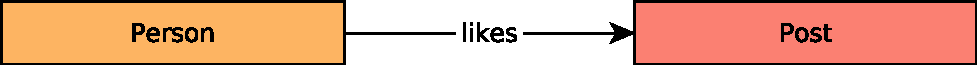
\includegraphics[scale=\patternscale,margin=0cm .2cm]{patterns/interactive-update-02}\hfill\vadjust{} \\ \hline
%
	desc. & Add a Like to a Post of the social network.
 \\ \hline
%
	
%
	
		params &
		\innerCardVSpace{\begin{tabularx}{\attributeCardWidth}{|>{\paramNumberCell}c|>{\varNameCell}M|>{\typeCell}m{\typeWidth}|Y|} \hline
		$\mathsf{1}$ & Person.id & ID &  \\ \hline
		$\mathsf{2}$ & Post.id & ID &  \\ \hline
		$\mathsf{3}$ & Person-likes->.creationDate & DateTime &  \\ \hline
		\end{tabularx}}\innerCardVSpace \\ \hline
	
%
	
%
	%
	%
	%
	%
\end{tabularx}
\queryCardVSpace